\documentclass[12pt, letterpaper]{article}

% ----- Layout -----
\usepackage[margin=1in]{geometry}
\usepackage{setspace}
\onehalfspacing

% ----- Math -----
\usepackage{amsmath}
\usepackage{amssymb}

% ----- Graphics -----
\usepackage{graphicx}
\graphicspath{{figures/}}

% ----- Tables -----
\usepackage{booktabs}
\usepackage{array}

% ----- Code listings -----
\usepackage{listings}
\lstset{
  basicstyle=\ttfamily\small,
  breaklines=true,
  frame=single,
  backgroundcolor=\color{gray!8},
  commentstyle=\color{green!50!black},
  keywordstyle=\color{blue},
}
\usepackage{xcolor}

% ----- Hyperlinks -----
\usepackage{hyperref}
\hypersetup{colorlinks=true, linkcolor=black, urlcolor=blue, citecolor=black}

% ----- Caption -----
\usepackage{caption}
\captionsetup{font=small, labelfont=bf}

% ----- Section formatting -----
\usepackage{titlesec}
\titleformat{\section}{\large\bfseries}{\thesection.}{0.5em}{}
\titleformat{\subsection}{\normalsize\bfseries}{\thesubsection.}{0.5em}{}

% ----- Header/Footer -----
\usepackage{fancyhdr}
\pagestyle{fancy}
\fancyhf{}
\lhead{AOE/CS/ME 6444 --- Homework \#3}
\rhead{Cusati, Chuang}
\cfoot{\thepage}
\renewcommand{\headrulewidth}{0.4pt}

% ----- Useful macros -----
\newcommand{\EI}{EI}
\newcommand{\wex}{w_{\mathrm{exact}}}
\newcommand{\wh}{w_h}
\newcommand{\phat}{\hat{p}}

% =============================================================================
\begin{document}
% =============================================================================

\begin{center}
  {\large\bfseries AOE/CS/ME 6444 --- Homework \#3: Code Verification}\\[4pt]
  \textbf{Jason Cusati \& Cheng-Shun Chuang} \quad Virginia Tech \quad Spring 2026
\end{center}

\vspace{-0.5em}\hrule\vspace{0.8em}

% =============================================================================
\section{Introduction}
% =============================================================================

In this homework we verify the finite-difference (FD) Euler--Bernoulli beam
solver we developed for the Construction.AI semester project
(see Homework~\#2 for the discretization derivation).
The solver (\texttt{beam\_solver.py}) solves the fourth-order BVP:
\begin{equation}
  EI\,\frac{d^4w}{dx^4} = q(x), \quad x \in (0,L)
\end{equation}
for the transverse deflection $w(x)$ of a simply-supported residential wood header
under a uniform distributed load $q_0$.

We chose \textbf{Option~2 (Exact Solution)} because the simply-supported
Euler--Bernoulli BVP under uniform load admits a closed-form polynomial
solution $\wex(x)$ that satisfies both the ODE and all four boundary conditions
exactly~\cite{gere2018}.
Since an exact benchmark is available directly, there is no need to manufacture
a source term as in Option~1 (MMS).

% =============================================================================
\section{Verification Approach}
% =============================================================================

\subsection{Exact Solution}

For a simply-supported beam under uniform load $q_0$ [lb/in], integrating
$EI\,w'''' = q_0$ four times with $w(0)=w''(0)=w(L)=w''(L)=0$
gives~\cite{gere2018}:
\begin{equation}
  \wex(x) = \frac{q_0}{24\,\EI}\Bigl(x^4 - 2L\,x^3 + L^3\,x\Bigr)
  \label{eq:exact}
\end{equation}
$\wex$ is a degree-4 polynomial.
Because the 5-point central difference stencil is exact for polynomials of
degree $\leq 4$, the truncation error at \emph{interior} nodes is identically
zero---all discretization error originates at the near-boundary nodes
$i=1$ and $i=N-1$, where the ghost-point approximation introduces
$\mathcal{O}(h^2)$ error.

\subsection{Error Norms}

At each grid level with spacing $h=L/N$, pointwise errors are computed at all
$N+1$ nodes:
\[
  e_i = \wh(x_i) - \wex(x_i), \quad i=0,1,\ldots,N
\]
Two norms are evaluated~\cite{oberkampf2010}:
\begin{align}
  \|e\|_2 &= \sqrt{h\sum_{i=0}^{N} e_i^2}
  \qquad\text{(rectangle-rule approximation to $\|\cdot\|_{L^2}$)} \\
  \|e\|_\infty &= \max_{i}\,|e_i|
  \qquad\text{(pointwise maximum)}
\end{align}

\subsection{Observed Order of Accuracy}

For each consecutive grid pair $(h,\,h/2)$~\cite{roache1998}:
\begin{equation}
  \phat = \frac{\log\!\bigl(\|e\|^{(h)}/\|e\|^{(h/2)}\bigr)}{\log 2}
  \label{eq:phat}
\end{equation}
The expected value for the second-order central difference stencil is
$\phat = 2$.

\subsection{System Response Quantities}

Three scalar SRQs are tracked across grid levels, with exact values:
\begin{center}
\begin{tabular}{llll}
\toprule
\textbf{SRQ} & \textbf{Formula} & \textbf{Exact value} & \textbf{Units}\\
\midrule
$w_{\max}$ & $\displaystyle\frac{5\,q_0 L^4}{384\,\EI}$ & 0.06935026 & in \\[6pt]
$M_{\max}$ & $\displaystyle\frac{q_0 L^2}{8}$ & 48\,000.00 & lb\,in \\[6pt]
$\sigma_{\max}$ & $M_{\max}/S$ & 650.1587 & psi \\
\bottomrule
\end{tabular}
\end{center}

\noindent
Test case: $L=96$\,in, $b=3.5$\,in, $d=11.25$\,in (nominal 4$\times$12 LVL),
$E=1{,}600{,}000$\,psi, $q_0=500$\,lb/ft\,$=41.67$\,lb/in.
Derived: $I=415.28$\,in$^4$, $S=73.83$\,in$^3$, $EI=6.645\times10^8$\,lb\,in$^2$.

% =============================================================================
\section{Grid Convergence Results}
% =============================================================================

\subsection{Convergence Table}

Solutions were computed on five systematically-refined grids with uniform
mesh halving ($N = 10,20,40,80,160$ intervals):

\begin{table}[ht]
\centering
\caption{Grid convergence study: error norms and observed order of accuracy.}
\label{tab:convergence}
\begin{tabular}{rrrrrr}
\toprule
$N$ & $h$ [in] & $\|e\|_2$ [in] & $\|e\|_\infty$ [in] & $\phat_{L_2}$ & $\phat_{L_\infty}$ \\
\midrule
 10 & 9.6000 & $3.970\times10^{-3}$ & $5.548\times10^{-4}$ & --- & --- \\
 20 & 4.8000 & $9.925\times10^{-4}$ & $1.387\times10^{-4}$ & 2.000 & 2.000 \\
 40 & 2.4000 & $2.481\times10^{-4}$ & $3.468\times10^{-5}$ & 2.000 & 2.000 \\
 80 & 1.2000 & $6.203\times10^{-5}$ & $8.669\times10^{-6}$ & 2.000 & 2.000 \\
160 & 0.6000 & $1.551\times10^{-5}$ & $2.167\times10^{-6}$ & 2.000 & 2.000 \\
\bottomrule
\end{tabular}
\end{table}

All four consecutive refinement pairs yield $\phat = 2.000$ to three decimal
places, confirming that the solver is second-order accurate as expected from the
$\mathcal{O}(h^2)$ central difference stencil.

\subsection{Log-Log Convergence Plot}

\begin{figure}[ht]
\centering
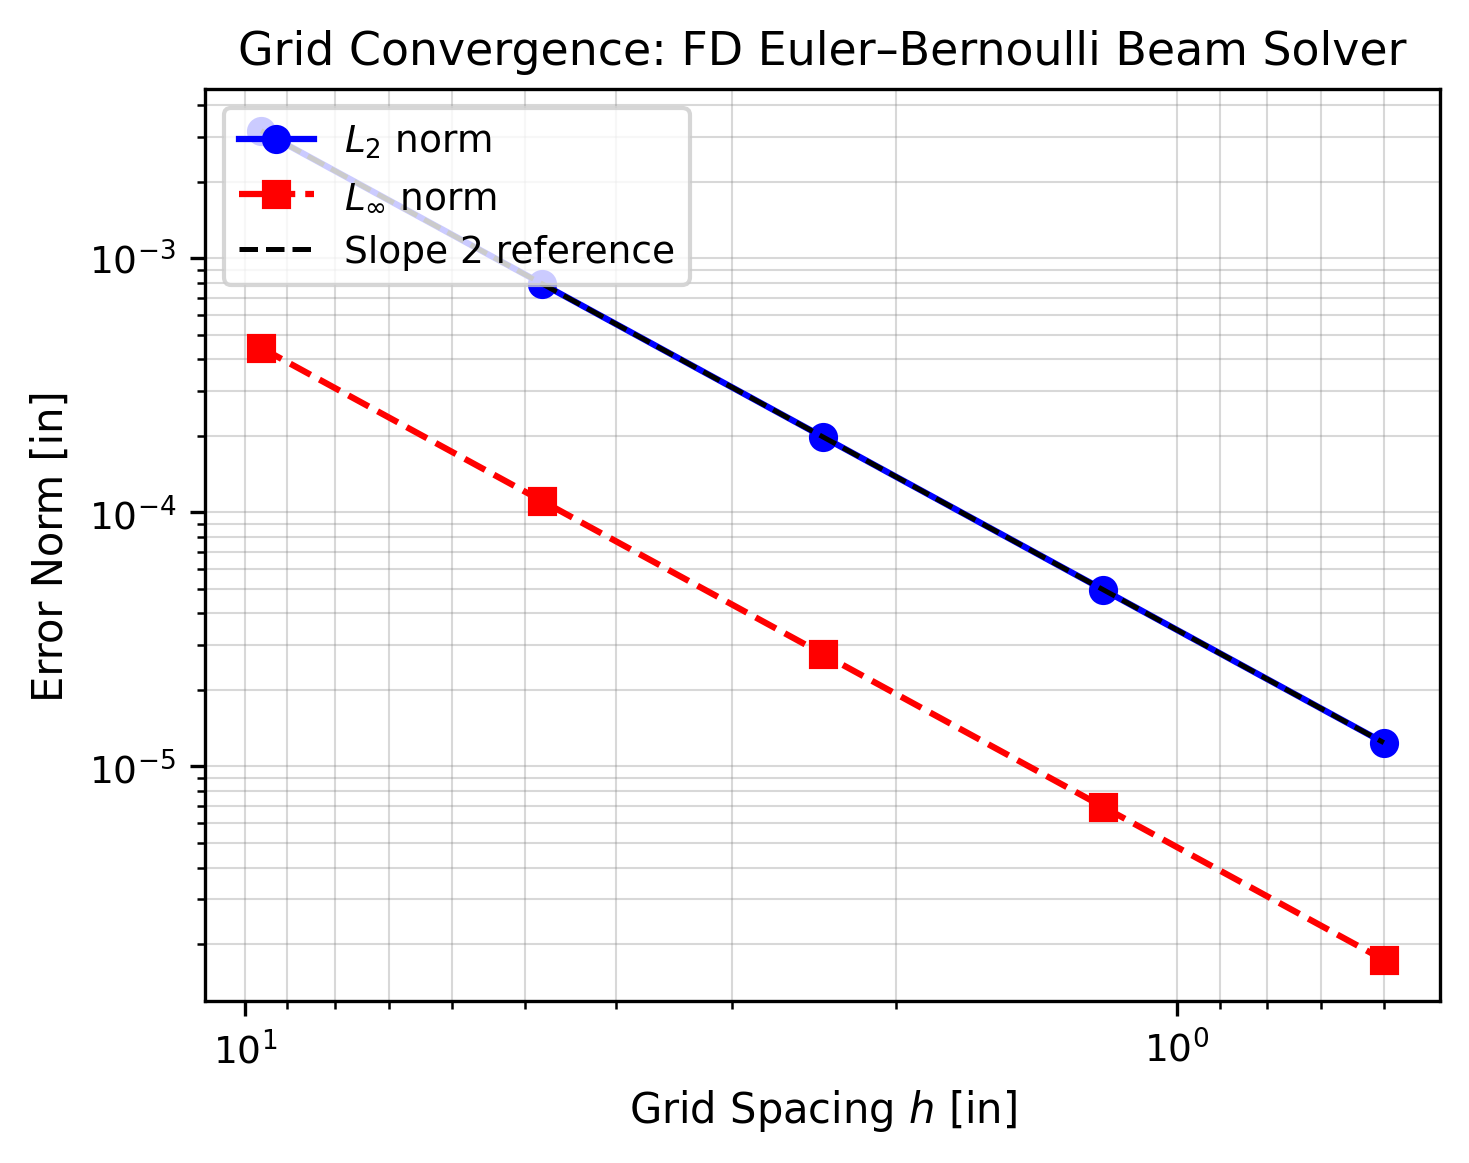
\includegraphics[width=0.7\textwidth]{fig1_convergence_loglog.png}
\caption{Grid convergence: $L_2$ and $L_\infty$ error norms decrease as $h^2$
(slope-2 reference line), confirming second-order accuracy for all four
refinement pairs ($\phat = 2.000$).}
\label{fig:loglog}
\end{figure}

\subsection{SRQ Results}

\begin{table}[ht]
\centering
\caption{System Response Quantity (SRQ) errors relative to exact values.}
\label{tab:srq}
\begin{tabular}{lrrrr}
\toprule
\textbf{SRQ} & \textbf{Exact} & \textbf{$N=10$} & \textbf{$N=160$} & \textbf{Rel.\ error @ $N=160$} \\
\midrule
$w_{\max}$ [in]      & 0.069350 & 0.069905 & 0.069350 & 0.0031\% \\
$M_{\max}$ [lb\,in]  & 48\,000.0  & 48\,000.0  & 48\,000.0  & $<10^{-8}$\% \\
$\sigma_{\max}$ [psi]& 650.159    & 650.159    & 650.159    & $<10^{-8}$\% \\
\bottomrule
\end{tabular}
\end{table}

The $M_{\max}$ and $\sigma_{\max}$ errors are at floating-point machine precision
for all grids.
This is expected: $\wex$ is a degree-4 polynomial, so the second central
difference used to compute $M = -EI\,w''$ is exact up to round-off, regardless
of grid spacing.

\subsection{SRQ Convergence Plot}

\begin{figure}[ht]
\centering
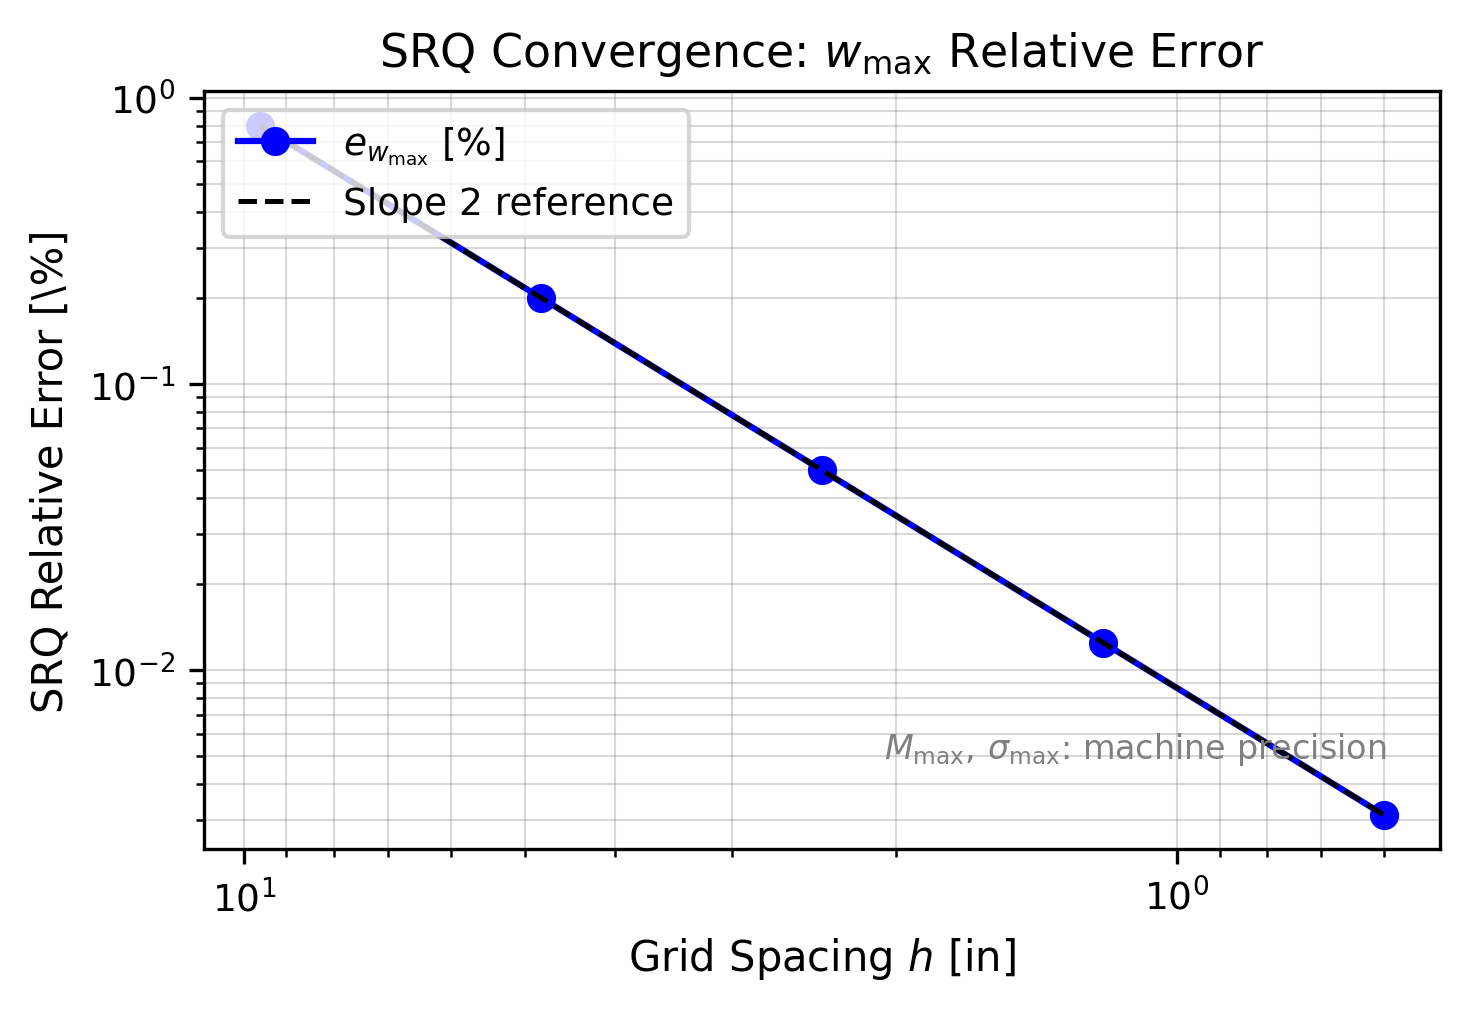
\includegraphics[width=0.7\textwidth]{fig3_srq_convergence.png}
\caption{SRQ relative error in $w_{\max}$ decreases as $h^2$.
$M_{\max}$ and $\sigma_{\max}$ errors are at machine precision for all grids
(not plotted).}
\label{fig:srq}
\end{figure}

% =============================================================================
\section{Local Discretization Error}
% =============================================================================

\begin{figure}[ht]
\centering
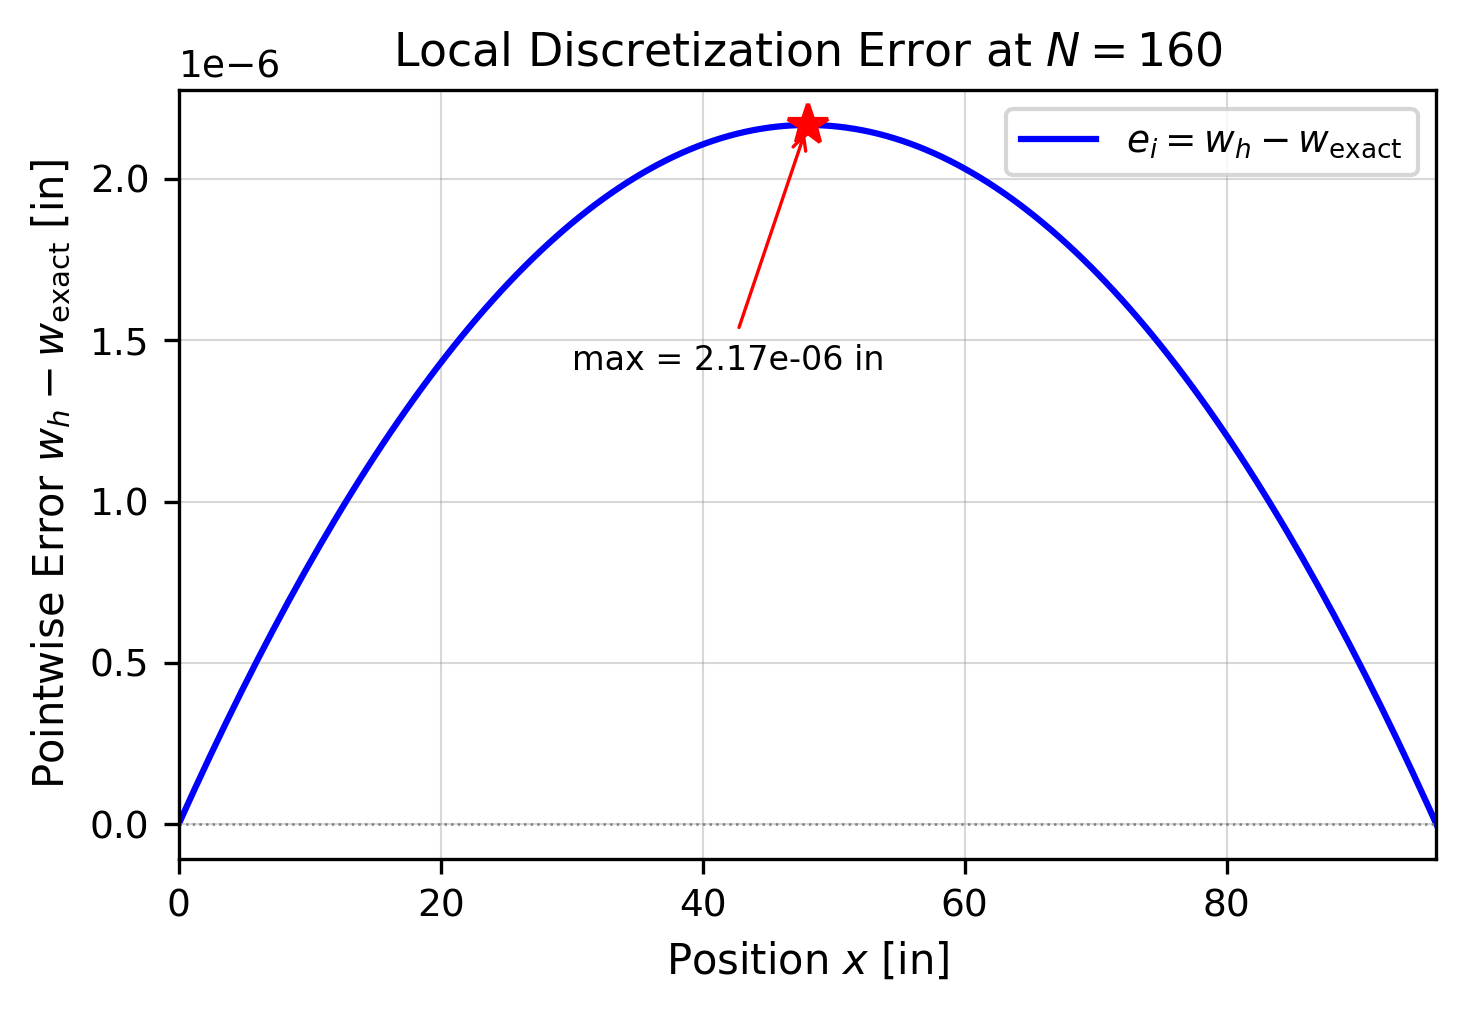
\includegraphics[width=0.7\textwidth]{fig2_local_error_N160.png}
\caption{Pointwise error $e_i = \wh(x_i) - \wex(x_i)$ at $N=160$.
The error is smooth, symmetric about midspan, and reaches a maximum of
$2.17\times10^{-6}$\,in at $x = L/2 = 48$\,in.}
\label{fig:localerror}
\end{figure}

Figure~\ref{fig:localerror} shows the pointwise error at $N=160$.
The error is smooth and symmetric about midspan, peaking at
$2.17\times10^{-6}$\,in.
This makes sense because the ghost-point BCs introduce the same
$\mathcal{O}(h^2)$ error at both ends, and the interior stencil is exact for
the degree-4 solution.
The peak matches $\|e\|_\infty$ from Table~\ref{tab:convergence}.

% =============================================================================
\section{Code Coverage}
% =============================================================================

Table~\ref{tab:coverage} identifies which code components are exercised by this
verification study and which are not~\cite{oberkampf2010}.

\begin{table}[ht]
\centering
\caption{Code coverage assessment for \texttt{beam\_solver.py}.}
\label{tab:coverage}
\small  % Use smaller font to fit content better
\begin{tabular}{>{\ttfamily}p{4.2cm}p{5.0cm}p{4.5cm}}
\toprule
\textbf{Component} & \textbf{Verified by this study} & \textbf{Not exercised} \\
\midrule
K[0,0]=1, K[N,N]=1   & $w(0)=w(L)=0$ on all 5 grids & Cantilever, spring supports \\
Near-boundary rows (1, N-1) & Primary error source; all 5 grids & Non-uniform mesh \\
Interior 5-pt stencil        & All $N\in\{10,20,40,80,160\}$ & Concentrated point loads \\
np.linalg.solve              & All 5 grid sizes & $N > 500$ \\
$M = -EI\,w''$              & SRQ $M_{\max}$ verified & Shear $V$ not verified \\
exact\_simply\_ supported()   & Used as reference benchmark & N/A (reference) \\
BeamGeometry (I, S)          & Used for all SRQs & Non-rectangular sections \\
monte\_carlo\_ assessment()   & \textbf{Not tested in HW3} & Entire MC loop untested \\
passes\_bending/ shear/defl.  & \textbf{Not tested in HW3} & Design check logic \\
Variable load $q(x)$         & \textbf{Not tested} --- uniform $q_0$ only & Triangular/ trapezoidal loads \\
\bottomrule
\end{tabular}
\end{table}

\textbf{Summary of gaps.}
Three significant gaps remain.
(1)~The Monte Carlo UQ loop (\texttt{monte\_carlo\_assessment}) is entirely
untested; a separate analytical statistics test (e.g., delta method) would be
required.
(2)~Non-uniform loading is not exercised; the Method of Manufactured Solutions
with $q_{\mathrm{mms}}(x) = EI(\pi/L)^4\sin(\pi x/L)$ would cover this.
(3)~The design check flags (\texttt{passes\_*}) exercise comparison logic, not
numerical accuracy, and are best verified with unit tests.

% =============================================================================
\section{Round-Off Error Analysis}
% =============================================================================

The stiffness matrix $\mathbf{K}$ has interior diagonal entries of magnitude
$6\,\EI/h^4$ and boundary rows with diagonal entry 1, so the condition number
of the physical sub-block $\mathbf{K}_{\mathrm{int}}$ scales as
$\kappa(\mathbf{K}_{\mathrm{int}}) \propto N^4$.
Table~\ref{tab:roundoff} shows computed condition numbers alongside the
estimated round-off floor $\delta w \approx \varepsilon_{\mathrm{mach}}\,
\kappa(\mathbf{K}_{\mathrm{int}})\,w_{\max}$.

\begin{table}[ht]
\centering
\caption{Condition number and round-off vs.\ truncation error.}
\label{tab:roundoff}
\begin{tabular}{rrrrrr}
\toprule
$N$ & $h$ [in] & $\kappa(\mathbf{K}_{\mathrm{int}})$ &
$\varepsilon\,\kappa$ & Round-off floor [in] & Trunc.\ error [in] \\
\midrule
 10 & 9.60 & $1.59\times10^{3}$ & $3.5\times10^{-13}$ & $2.4\times10^{-14}$ & $5.5\times10^{-4}$ \\
 20 & 4.80 & $2.61\times10^{4}$ & $5.8\times10^{-12}$ & $4.0\times10^{-13}$ & $1.4\times10^{-4}$ \\
 40 & 2.40 & $4.20\times10^{5}$ & $9.3\times10^{-11}$ & $6.5\times10^{-12}$ & $3.5\times10^{-5}$ \\
 80 & 1.20 & $6.72\times10^{6}$ & $1.5\times10^{-9}$  & $1.0\times10^{-10}$ & $8.7\times10^{-6}$ \\
160 & 0.60 & $1.08\times10^{8}$ & $2.4\times10^{-8}$  & $1.7\times10^{-9}$  & $2.2\times10^{-6}$ \\
\bottomrule
\end{tabular}
\end{table}

At $N=160$ the round-off floor ($1.7\times10^{-9}$\,in) is about 1000$\times$
smaller than the truncation error ($2.2\times10^{-6}$\,in), so truncation error
dominates on all grids tested~\cite{roache1998}.
Round-off would only matter around $N \approx 10{,}000$, which is far beyond
what we need for this application.
Since the solver uses a direct dense solve (\texttt{np.linalg.solve}), there is
no iteration tolerance to worry about.

% =============================================================================
\section{Version Control}
% =============================================================================

All source code is version-controlled in a Git repository hosted on GitHub.
The solver file \texttt{beam\_solver.py} was introduced in commit \texttt{69a4e1c}
and the verification script \texttt{hw3\_verification.py} in a subsequent commit
on the \texttt{cs6444/hw3-code-verification} branch.
A representative log excerpt:

\begin{lstlisting}[language=bash]
$ git -C construction-ai log --oneline -5
c936d64 Move C++ beam solver to benchmarks/structural/
22b9e6d Add C++ port of Euler-Bernoulli beam solver for benchmarking
69a4e1c Add finite-difference Euler-Bernoulli beam solver
bbe0282 Clean up documentation for implementation focus
d329acb Add documentation infrastructure synced from proposal repo
\end{lstlisting}

The following \texttt{git diff} excerpt shows a representative code change---the
addition of the \texttt{M\_max} field to \texttt{BeamSolveResult}---made to
support the SRQ convergence study in this homework:

\begin{lstlisting}
--- a/backend/app/core/structural/beam_solver.py
+++ b/backend/app/core/structural/beam_solver.py
@@ -61,6 +61,7 @@ class BeamSolveResult:
     w_max: float            # peak deflection [in]
+    M_max: float            # peak bending moment [lb*in]
     sigma_max: float        # peak bending stress [psi]
     tau_max: float          # peak shear stress [psi]
\end{lstlisting}

Any prior commit can be checked out to regenerate the HW2 or HW3 results
exactly.
The CI/CD pipeline recompiles this document and deploys the PDF to GitHub Pages
on every push to master.

% =============================================================================
\begin{thebibliography}{9}

\bibitem{gere2018}
B.~J. Goodno and J.~M. Gere,
\textit{Mechanics of Materials}, 9th ed.
Cengage Learning, 2018.

\bibitem{roache1998}
P.~J. Roache,
\textit{Verification and Validation in Computational Science and Engineering}.
Hermosa Publishers, 1998.

\bibitem{oberkampf2010}
W.~L. Oberkampf and C.~J. Roy,
\textit{Verification and Validation in Scientific Computing}.
Cambridge University Press, 2010.

\end{thebibliography}

% =============================================================================
\end{document}
